% nnU-Net (PlainConvUNet, 3d_fullres) architecture — BraTS 2021
% 6 encoder stages: 128³→4³, 32→320 ch; 5 decoder stages; 2×(Conv3³+IN+LReLU)/stage
\documentclass[border=20pt, tikz]{standalone}
\usetikzlibrary{arrows.meta, calc}

\begin{document}
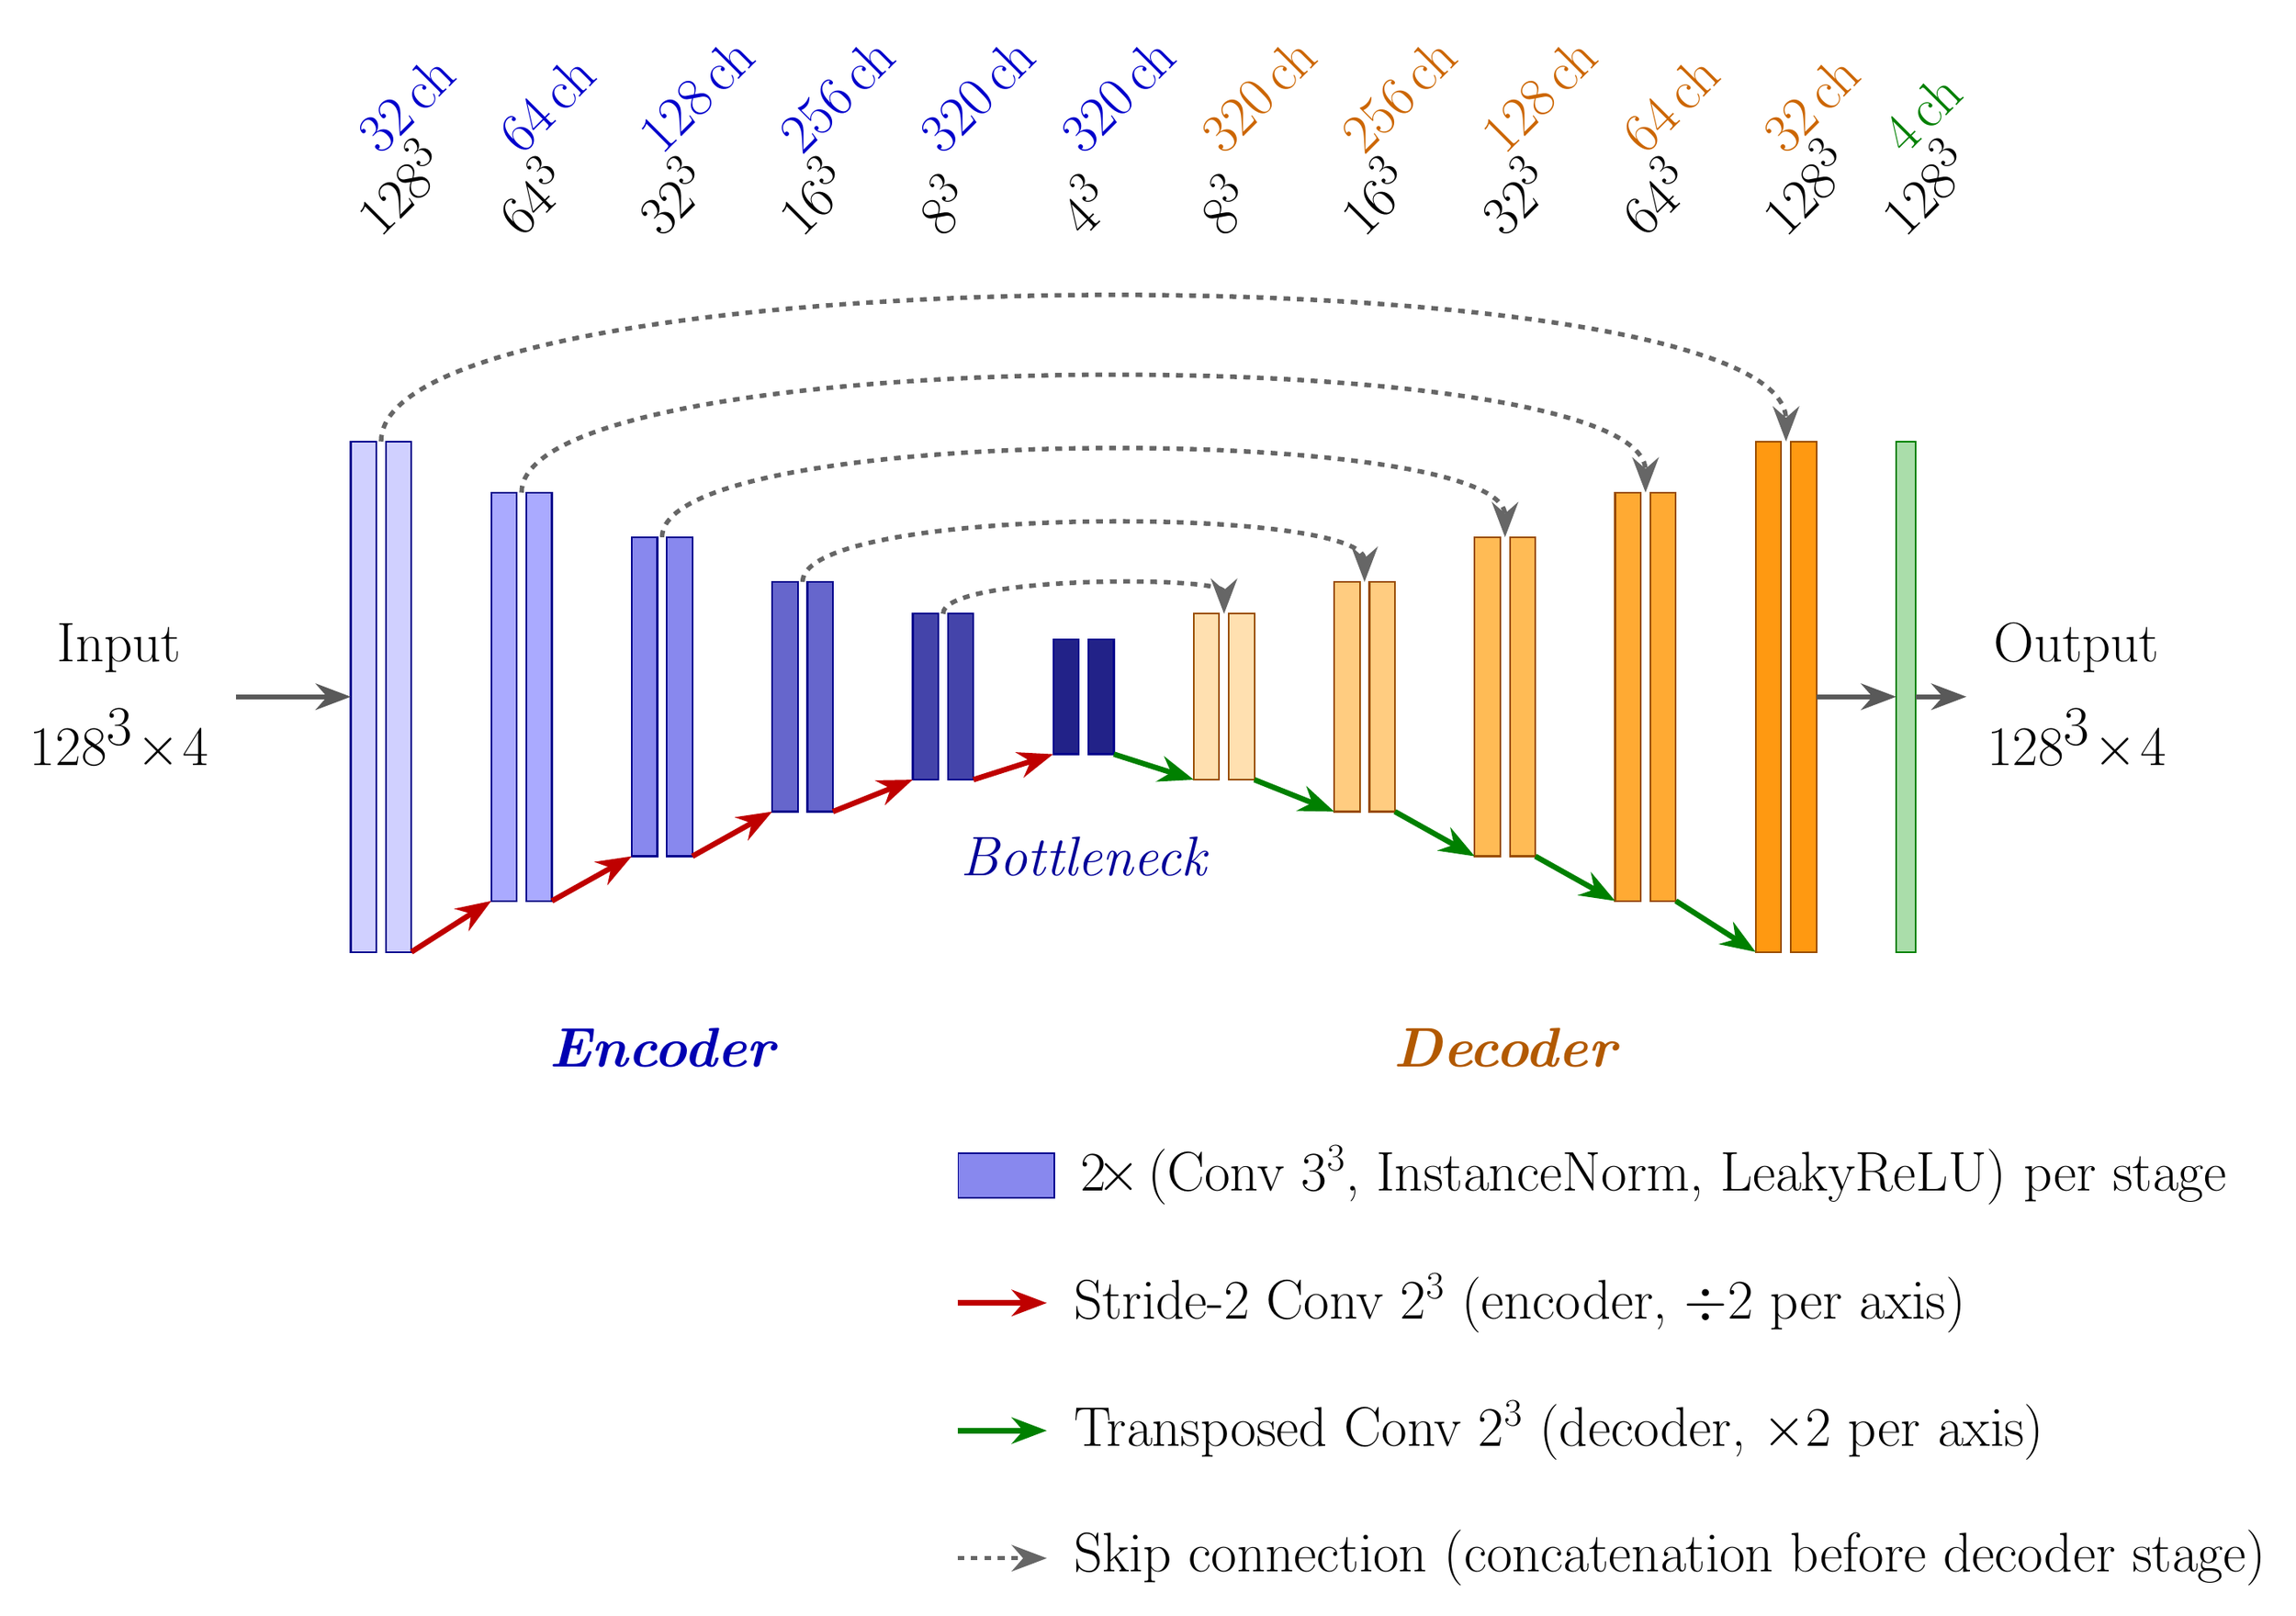
\begin{tikzpicture}[
  font=\fontsize{35}{42}\selectfont,
  pool/.style  = {-{Stealth[length=5.5mm]}, line width=2.4pt, draw=red!75!black},
  up/.style    = {-{Stealth[length=5.5mm]}, line width=2.4pt, draw=green!50!black},
  skip/.style  = {-{Stealth[length=5.5mm]}, line width=2.0pt, draw=black!60, dashed},
  arr/.style   = {-{Stealth[length=5.5mm]}, line width=2.2pt, draw=black!65},
]

% ── Color definitions ─────────────────────────────────────────────────────────
\definecolor{enc1c}{HTML}{D0D0FF}
\definecolor{enc2c}{HTML}{AAAAFF}
\definecolor{enc3c}{HTML}{8888EE}
\definecolor{enc4c}{HTML}{6666CC}
\definecolor{enc5c}{HTML}{4444AA}
\definecolor{enc6c}{HTML}{222288}
\definecolor{dec1c}{HTML}{FF9911}
\definecolor{dec2c}{HTML}{FFAA33}
\definecolor{dec3c}{HTML}{FFBB55}
\definecolor{dec4c}{HTML}{FFCC80}
\definecolor{dec5c}{HTML}{FFE0B0}
\definecolor{outcc}{HTML}{AADDAA}
\colorlet{enc_edge}{blue!55!black}
\colorlet{dec_edge}{orange!60!black}

% ── Stage macro ───────────────────────────────────────────────────────────────
% \mkstage{name}{x_left}{half_height}{fill}{edge}
% Two rects, centered at y=0, each 0.40 cm wide, 0.15 cm gap => pair total 0.95 cm
\newcommand{\mkstage}[5]{%
  \filldraw[fill=#4, draw=#5, line width=0.8pt]
    (#2, {-#3}) rectangle ++(0.40, {2*#3});
  \filldraw[fill=#4, draw=#5, line width=0.8pt]
    ({#2+0.55}, {-#3}) rectangle ++(0.40, {2*#3});
  \coordinate (#1-nw) at (#2,        {#3});
  \coordinate (#1-ne) at ({#2+0.95}, {#3});
  \coordinate (#1-sw) at (#2,        {-#3});
  \coordinate (#1-se) at ({#2+0.95}, {-#3});
  \coordinate (#1-n)  at ({#2+0.475},{#3});
  \coordinate (#1-s)  at ({#2+0.475},{-#3});
  \coordinate (#1-e)  at ({#2+0.95}, 0);
  \coordinate (#1-w)  at (#2, 0);
}

% ── Encoder: 6 stages, 2.2 cm apart ──────────────────────────────────────────
\mkstage{e1}{ 0.0}{4.00}{enc1c}{enc_edge}  % 128^3 /  32 ch
\mkstage{e2}{ 2.2}{3.20}{enc2c}{enc_edge}  %  64^3 /  64 ch
\mkstage{e3}{ 4.4}{2.50}{enc3c}{enc_edge}  %  32^3 / 128 ch
\mkstage{e4}{ 6.6}{1.80}{enc4c}{enc_edge}  %  16^3 / 256 ch
\mkstage{e5}{ 8.8}{1.30}{enc5c}{enc_edge}  %   8^3 / 320 ch
\mkstage{e6}{11.0}{0.90}{enc6c}{enc_edge}  %   4^3 / 320 ch  (bottleneck)

% ── Decoder: 5 stages, same spacing ──────────────────────────────────────────
\mkstage{d5}{13.2}{1.30}{dec5c}{dec_edge}  %   8^3 / 320 ch
\mkstage{d4}{15.4}{1.80}{dec4c}{dec_edge}  %  16^3 / 256 ch
\mkstage{d3}{17.6}{2.50}{dec3c}{dec_edge}  %  32^3 / 128 ch
\mkstage{d2}{19.8}{3.20}{dec2c}{dec_edge}  %  64^3 /  64 ch
\mkstage{d1}{22.0}{4.00}{dec1c}{dec_edge}  % 128^3 /  32 ch

% ── Output conv (thin green slab, same height as d1) ─────────────────────────
\filldraw[fill=outcc, draw=green!50!black, line width=0.8pt]
  (24.2, -4.00) rectangle ++(0.30, 8.00);
\coordinate (out-w) at (24.20, 0);
\coordinate (out-e) at (24.50, 0);
\coordinate (out-n) at (24.35, 4.00);

% ── Encoder downsampling arrows (stride-2 conv) ───────────────────────────────
\draw[pool] (e1-se) -- (e2-sw);
\draw[pool] (e2-se) -- (e3-sw);
\draw[pool] (e3-se) -- (e4-sw);
\draw[pool] (e4-se) -- (e5-sw);
\draw[pool] (e5-se) -- (e6-sw);

% ── Decoder upsampling arrows (transposed conv) ───────────────────────────────
\draw[up] (e6-se) -- (d5-sw);
\draw[up] (d5-se) -- (d4-sw);
\draw[up] (d4-se) -- (d3-sw);
\draw[up] (d3-se) -- (d2-sw);
\draw[up] (d2-se) -- (d1-sw);

% ── Skip connections: smooth arcs above (same looseness => wider=higher) ──────
% Arc peak ≈ hh + 0.25 * 0.35 * chord:
%   e5<->d5: chord=4.4  => peak 1.69   e4<->d4: 8.8  => 2.57
%   e3<->d3: chord=13.2 => peak 3.66   e2<->d2: 17.6 => 4.74
%   e1<->d1: chord=22.0 => peak 5.93   (labels placed at y >= 7.0)
\draw[skip] (e5-n) to[out=90,in=90,looseness=0.35] (d5-n);
\draw[skip] (e4-n) to[out=90,in=90,looseness=0.35] (d4-n);
\draw[skip] (e3-n) to[out=90,in=90,looseness=0.35] (d3-n);
\draw[skip] (e2-n) to[out=90,in=90,looseness=0.35] (d2-n);
\draw[skip] (e1-n) to[out=90,in=90,looseness=0.35] (d1-n);

% ── Input / Output flow ───────────────────────────────────────────────────────
\draw[arr] (-1.8,  0) -- (e1-w);
\draw[arr] (d1-e)     -- (out-w);
\draw[arr] (out-e)    -- (25.3, 0);

\node[align=center, anchor=east] at (-2.1, 0)  {Input\\[4pt]$128^3\!\times\!4$};
\node[align=center, anchor=west] at (25.5, 0)  {Output\\[4pt]$128^3\!\times\!4$};

% ── Resolution + channel labels (fixed y above arcs, rotated 45 deg) ──────────
\node[rotate=45,anchor=south west,font=\fontsize{29}{35}\selectfont] at ( 0.475,7.0){$128^3$};
\node[rotate=45,anchor=south west,font=\fontsize{29}{35}\selectfont,color=blue!80!black] at ( 0.475,8.3){32\,ch};
\node[rotate=45,anchor=south west,font=\fontsize{29}{35}\selectfont] at ( 2.675,7.0){$64^3$};
\node[rotate=45,anchor=south west,font=\fontsize{29}{35}\selectfont,color=blue!80!black] at ( 2.675,8.3){64\,ch};
\node[rotate=45,anchor=south west,font=\fontsize{29}{35}\selectfont] at ( 4.875,7.0){$32^3$};
\node[rotate=45,anchor=south west,font=\fontsize{29}{35}\selectfont,color=blue!80!black] at ( 4.875,8.3){128\,ch};
\node[rotate=45,anchor=south west,font=\fontsize{29}{35}\selectfont] at ( 7.075,7.0){$16^3$};
\node[rotate=45,anchor=south west,font=\fontsize{29}{35}\selectfont,color=blue!80!black] at ( 7.075,8.3){256\,ch};
\node[rotate=45,anchor=south west,font=\fontsize{29}{35}\selectfont] at ( 9.275,7.0){$8^3$};
\node[rotate=45,anchor=south west,font=\fontsize{29}{35}\selectfont,color=blue!80!black] at ( 9.275,8.3){320\,ch};
\node[rotate=45,anchor=south west,font=\fontsize{29}{35}\selectfont] at (11.475,7.0){$4^3$};
\node[rotate=45,anchor=south west,font=\fontsize{29}{35}\selectfont,color=blue!80!black] at (11.475,8.3){320\,ch};
\node[rotate=45,anchor=south west,font=\fontsize{29}{35}\selectfont] at (13.675,7.0){$8^3$};
\node[rotate=45,anchor=south west,font=\fontsize{29}{35}\selectfont,color=orange!80!black] at (13.675,8.3){320\,ch};
\node[rotate=45,anchor=south west,font=\fontsize{29}{35}\selectfont] at (15.875,7.0){$16^3$};
\node[rotate=45,anchor=south west,font=\fontsize{29}{35}\selectfont,color=orange!80!black] at (15.875,8.3){256\,ch};
\node[rotate=45,anchor=south west,font=\fontsize{29}{35}\selectfont] at (18.075,7.0){$32^3$};
\node[rotate=45,anchor=south west,font=\fontsize{29}{35}\selectfont,color=orange!80!black] at (18.075,8.3){128\,ch};
\node[rotate=45,anchor=south west,font=\fontsize{29}{35}\selectfont] at (20.275,7.0){$64^3$};
\node[rotate=45,anchor=south west,font=\fontsize{29}{35}\selectfont,color=orange!80!black] at (20.275,8.3){64\,ch};
\node[rotate=45,anchor=south west,font=\fontsize{29}{35}\selectfont] at (22.475,7.0){$128^3$};
\node[rotate=45,anchor=south west,font=\fontsize{29}{35}\selectfont,color=orange!80!black] at (22.475,8.3){32\,ch};
\node[rotate=45,anchor=south west,font=\fontsize{29}{35}\selectfont] at (24.35, 7.0){$128^3$};
\node[rotate=45,anchor=south west,font=\fontsize{29}{35}\selectfont,color=green!50!black] at (24.35, 8.3){4\,ch};

% ── Bottleneck / section labels ───────────────────────────────────────────────
\node[font=\fontsize{32}{38}\selectfont\itshape, color=blue!60!black]
  at (11.475, -2.5) {\itshape Bottleneck};
\node[font=\fontsize{37}{44}\selectfont\bfseries\itshape, color=blue!70!black]
  at (4.875, -5.5) {\textbf{\textit{Encoder}}};
\node[font=\fontsize{37}{44}\selectfont\bfseries\itshape, color=orange!70!black]
  at (18.075, -5.5) {\textbf{\textit{Decoder}}};

% ── Legend (bottom-right) ─────────────────────────────────────────────────────
\def\LY{-7.5}   % top row y
\def\LS{2.0}    % vertical spacing between legend rows
\def\LX{9.5}    % left x (bottom-right alignment)

% Row 1: encoder/decoder conv block swatch
\node[draw=enc_edge, fill=enc3c, line width=0.7pt,
      minimum width=1.5cm, minimum height=0.7cm, anchor=west] at (\LX, \LY) {};
\node[font=\fontsize{25}{30}\selectfont, anchor=west] at ({\LX+1.8}, \LY)
  {$2\!\times\!$ (Conv $3^3$, InstanceNorm, LeakyReLU) per stage};

% Row 2: downsampling arrow
\draw[pool] (\LX, {\LY-\LS}) -- ++(1.4, 0);
\node[font=\fontsize{25}{30}\selectfont, anchor=west] at ({\LX+1.7}, {\LY-\LS})
  {Stride-2 Conv $2^3$ (encoder, $\div 2$ per axis)};

% Row 3: upsampling arrow
\draw[up] (\LX, {\LY-2*\LS}) -- ++(1.4, 0);
\node[font=\fontsize{25}{30}\selectfont, anchor=west] at ({\LX+1.7}, {\LY-2*\LS})
  {Transposed Conv $2^3$ (decoder, $\times 2$ per axis)};

% Row 4: skip connection
\draw[skip] (\LX, {\LY-3*\LS}) -- ++(1.4, 0);
\node[font=\fontsize{25}{30}\selectfont, anchor=west] at ({\LX+1.7}, {\LY-3*\LS})
  {Skip connection (concatenation before decoder stage)};

\end{tikzpicture}
\end{document}
